\documentclass [12pt, oneside] {book}

\usepackage{amssymb}
\renewcommand{\baselinestretch}{1.5}
\usepackage[utf8]{inputenc}
\usepackage{geometry}
\geometry{a4paper, portrait, margin=2.5cm}
\usepackage[round]{natbib}
\usepackage{graphicx} %package to manage images
\usepackage{dirtytalk}
\graphicspath{ {./images/} }
%\usepackage[rightcaption]{sidecap}
\usepackage[font=scriptsize, labelfont=bf]{caption}
\usepackage{wrapfig}
\usepackage{hyperref}
\usepackage[acronym, toc]{glossaries}
\usepackage{acronym} 
\usepackage[nottoc]{tocbibind}
\makeglossaries


\begin{document}
\begin{titlepage}
    \begin{center}
        \vspace*{1cm}
        \Huge
        \textbf{Participatory Action Research in Virtual Reality: Virtual Time-Machine tour}
        \vfill
        \LARGE
        \textbf{Master Thesis}
        
        \vspace{0.5cm}
        submitted by:
        \vspace{1.5cm}
        \textbf{Samer Shawar}\\
        Matriculation Number: 1380673
        \vfill
        \textit {First Examiner: Prof. Dr. Volker Wulf}
        
        
        \textit {Second Examiner: Prof. Dr. Markus Rohde}
        \vfill
        %\vspace{0.8cm}
        \Large
        Human Computer Interaction\\
        University of Siegen\\
        October 2019\\
 \end{center}
\end{titlepage}
\pagenumbering{Roman}
\addcontentsline{toc}{section}{Acknowledgement}
\section*{Acknowledgement}
bla bla bla bla
\newpage
\section*{Abstract}
Since 1948, the Palestinian refugees are not allowed to go back to Palestine. The existence of the Israeli state prevented the Palestinian refugees to get back to their homes. Their houses and villages were depopulated and demolished. Traveling to Palestine could be intimidating for some people due to the perception that the western media have shown about the country. Palestinian refugees need to have access to see Palestine. Anybody who wants to visit the country, but has political situation concerns, must experience or see what to expect of a visit to Palestine. Action research was the concept of developing Glimpses from Palestine \acrlong{vr} application. The application development was based on the insights that were collected from interviews. The rebuilding of one of the demolished villages in \acrlong{vr} has given the application a historical and political aspect. The results show a strong connection between the second and third generations of Palestinians and Palestine. The transition of stories from grandparents to grandchildren in the diaspora and their effect on maintaining a strong relationship with the country. Also, the results showed the effect that Glimpses from Palestine has on people to preserve the value of their country and villages. This research explores the \acrlong{vr} as a new approach for documenting and displaying the historical events and facts of a country as Palestine, that the history and the demography of the country were changed due to political conflict. 
\addcontentsline{toc}{section}{Abstract}
\tableofcontents
\listoffigures

\newacronym{vr}{VR}{Virtual Reality}
\newacronym{ui}{UI}{User Interface}
\newacronym{yallah!}{YALLAH!}{You all are hackers!}
\newacronym{idf}{IDF}{Israel Defence Forces}
\newacronym{hmd}{HMD}{Head-Mounted Display}
\newacronym{pd}{PD}{Participatory Design}
\newacronym{pa}{PA}{Palestinian Authority}
\newacronym{unrwa}{UNRWA}{United Nations Relief and Works Agency for Palestine Refugees}
\newacronym{plo}{PLO}{Palestine Liberation Organization}
\newacronym{un}{UN}{United Nations}
\newacronym{jnf}{JNF}{Jewish National Fund}
\newacronym{ala}{ALA}{Arab Liberation Army}
\newacronym{fov}{FOV}{Field of View}
\newacronym{for}{FOR}{Field of Regard}
\newacronym{cave}{CAVE}{Cave Automatic Virtual Environment}
\newacronym{cad}{CAD}{Computer-Aided Design}

\printglossary[type=\acronymtype, title=Abbreviations, nonumberlist]


\chapter{Introduction}
\pagenumbering{arabic}
During the last decade the word ‘virtual’ became one of the most exposed words in the
English language, today we have virtual universities, virtual offices, virtual pets, virtual
studios, etc., and all of this because of virtual reality \acrshort{vr} \citep{Vince2011}. The \acrshort{vr} hit the
headline in the mid-1980’s and spawned a series of conferences, exhibitions, television
programs, and philosophical debates about the meaning of reality (Vince, 2011). “Virtual
reality is using a computer to create images of 3D scenes where the person can navigate and
interact” (Vince, 2011). Pinotti (2017) explained that immersivity and interactivity in virtual
environments are able to elicit in the user an intense feeling of “being there”, namely of being
embodied in an independent and self-referential world (Pinotti, 2017).

This master thesis will examine a virtual reality smart-phone application if it can let people overcome borders and if virtual reality can strengthen resilience for people by seeing their rebuilt villages in the virtual world. 


Virtual reality will need the development of the environment, according to the previous study at the Hackathon exchange program the users showed the interest of people for having a smart-phone application that allows them to experience the virtual reality at Palestine. For developing the application framework, a development environment like Unity Gaming engine will be used for improving the application due to the easy implementation of the Virtual Reality environment at Unity and the ability to distribute it over a variety of devices. Unity provides the ability to develop a virtual reality environment and Implement 3D models inside the real 360$^{\circ}$ videos.


Respectively for the maps and the data collected about the structure of the villages, the houses will be 3D modeled to rebuild a village or a part of it in the Virtual world. Blender will be used to create the 3D models of the houses and texture the buildings in the villages. Blender is an open-source 3D animation software, and it is structured for modeling and animation. The 3D modeled village will be integrated within the 360$^{\circ}$ video of the same village area. Points of interest will be distributed among the map of the village and the 360$^{\circ}$ video will be filmed from the same points of interest. The Villages actual locations will be filmed by a GoPro Fusion a 360$^{\circ}$ 5K camera. Through the prototype, the user will be able to see the actual location of the village nowadays, and will also have the option to see how was it pre-1948. 

The sound of the surrounding environment will immerse the user into the scenes, for interactivity between the user and the virtual environment, the user will have a gaze feature that allows commuting between the points of interest inside the village for instance. The gaze feature will be activated only when the user looks at the point of interest for a few seconds, a time-line will start moving to inform and prepare the user to be transferred to another scene. The user needs a virtual reality glasses to be able to get immersed in the application and see the whole environment. The virtual reality glasses are expensive and they need a very good computer to be able to operate them. Google created a VR lens out of cardboard, it allows the users to use their smart-phones as a display for the cardboard and experience virtual reality. The cardboard is easy to move with it and pass different checkpoints, airports, borders because it is only cardboard and it is also very cheap. That will make it easy for us to move around and show the application to different people and evaluate the application.

Participatory action research is best represented as a self-reflective
spiral of cycles of planning, acting and observing, reflecting and then re-planning in successive cycles of improvement \citep{KemmisSdanMcTaggart1988}. Participatory action research will allow us to evaluate the application with the participants and understand their concerns about their usability and interaction with the design. we will give the participants the prototype and let them test it, while we are observing how they interact and use the prototype, also we will let them reflect on the design and the product and take it for improvement in the design. Participatory action research will allow us to have a better evaluation from users to form a better action and interaction where the users had already conducted practice on the product. The evaluation will be taken by different participants from Palestinian refugees in Palestine, Jordan, and Lebanon, but also non-Palestinians will evaluate the application since the application is addressed for all people and see if Virtual reality can let them overcome borders.





The idea is to develop a new application to show Palestine with 360$^{\circ}$ videos, but it will include a part of one of the demolished villages before 1948. To rebuild one of those villages we need to know the structure of the village and how it looked like. The data about the structure of the village will be collected through personal stories, old pictures, British mandate aerial photos, and some maps made by a few people who lived in those villages. 
  
  
In the master project, a pre-study of the project will be conducted with Palestinians who live in the diaspora through interviews and workshops.  The Interview is a highly used method of collecting data in qualitative social research methods” \citep{Anyan2013}.  Kvale(1983)  described the purpose of as a method collection in social research as “... to gather descriptions of the life-world of the interviewee with respect to interpretation of the meaning of the described phenomena”  \citep{Kvale1983}. Semi-structured interviews will be used for collecting stories and exploring personal experiences about the Palestinians displacement and their relation with Palestine after living abroad. A questions guideline will be prepared for the interviews with  open-ended questions allowing a discussion with the interviewee rather than  formulated questions and answers.

After the interview some insights would be collected from the interviewee through a participatory design workshop. Participatory design (PD) is a set of theories, practices, and studies related to end-users as full participants in activities leading to software and hardware computer products and computer-based activities  \citep{Muller2003}. The field is extraordinarily diverse,  drawing on fields such as user-centered design, graphic design, software engineering, architecture, public policy, psychology, anthropology, sociology, labor studies, communication studies, and political science, and from localized experiences in diverse national and cultural contexts \citep{Gregory2003}.  Personal stories might give the ability for some refugees to draw the houses of their villages how they remember it. Applying a workshop for some of the Palestinian refugees to re-draw their houses would demonstrate a better image for the construction of the village, and that will give them the ability to tell us what they would like to see. houses, public places, walking paths between the houses, farms...etc. 
Information and communications technologies (ICT) artifacts should react to changing conditions of a social system \citep{Wulf2011}. Design case studies give us the ability to understand the relationship between social practice and the design of ICT artifacts that are built to support those practices, It is not so much about high tech, but about high-value \citep{Volker2013}. Design Case Studies ideally consist of three phases: (1) Analyze and particularly describe a social practice on a micro-level, as well describing the tools, media and their usage. (2) Describe the ICT artifacts from a product and from a process perspective, like the design concepts, and the applied design methods. (3) Document the introduction, appropriation and the potential re-design of the ICT artifact, documentation allows analyzing the trans-formative impact of certain functions and design options \citep{Volker2013}. Design case studies will allow us to check with the Palestinian refugees the tools or the practice that they do to see or to feel the connection with Palestine as a country and with their villages. After understanding their tools or practice, we can build a design depending on a specific design concept and methods. By letting them trying the prototype we will have general feedback about the interaction of the user with the App, and what would need to maintain and what kind of things needs to be re-designed. Design case studies will give us a general overview of the design concept and full fill us with the answers for the "how" and "why" about using the design methods.   
The Application will start by showing an overview of the whole map of historical Palestine. Points of interest will hover over the cities, the user will select a point of interest through the gaze feature. After selection, the map will be zoomed to the city location and will show more specified places within the city and the villages surrounding the city. The user will be transferred to a 360$^{\circ}$ video of the desired place, and inside the 360$^{\circ}$ video the user can commute inside the village for instance through the points of interest. sound of the surrounding environment will be added to the videos, as well as narrating the history and personal stories about the place. Within the demolished village, the user will have the ability to see how is the village look like now, and how it used to look like before 1948 by selecting an interactive button to travel in time. The user will have the ability to move back to the main map to choose to see different locations. All the methods that are used will help us to develop and collect the information and the data that is needed for the application and to be presented to the user.




The term virtual is becoming one of the most revealed words in the English language over the past decade, today we have virtual schools, virtual workplaces, virtual animals, virtual studios, etc \citep{Vince2011}.
A pre-study for a \acrfull{vr} smart-phone application that allows the users to visit Palestine without crossing any borders. Immersion and interactivity in virtual environments will give the user a profound feeling of \say{being there} that is, expressed in an individual and self-referential world (Pinotti, 2017). As a case study, Al-Ghabisiyya a Palestinian village that has been depopulated and demolished has been re-modeled and placed in the application. Therefore the user can travel back in time and see Palestine before 1948. Multiple platforms and applications are doing a similar purpose. Therefore I show a comparison between those platforms and applications to the application that I built. Then I will explain the research gap that I found through my pre-study, and how the application reduced the research gap. A detailed history timeline explained for understanding the setting of the research field and the problem that the application would help to solve. I will explain how this application developed from an idea that came out at a student exchange program \acrfull{yallah!} between the University of Siegen in Germany and the University of Birzeit in Palestine. The followed chapter will present the methodological approach of the research and how I conducted each method to collect data from the users and the field.  


\chapter{State of the Art}

  
Virtual reality is a technology which is often regarded as a natural extension to 3D computer graphics with advanced input and output devices \citep{Jayaram1997}. Ryan (2001) defined it as an “interactive, immersive experience generated by a computer” \citep{Ryan2001}. And according to G.C. Burdea and Coiffet (2017) “it is a generated computer graphics used to create a realistic-looking world that responds to the user’s input (gestures, verbal commands, etc.)” \citep{burdea2017virtual}. Virtual reality places the users inside the experience instead of viewing a screen in front of them, the users will be immersed inside a 3D world. As shown in Figure \ref{fig:3I} Three elements are needed to construct a virtual reality situation: immersion, interaction, and imagination. They are called the “3I’s” of virtual reality \citep{Hu2016}.


\begin{wrapfigure}{r}{0.30\textwidth} %this figure will be at the left
    \centering
    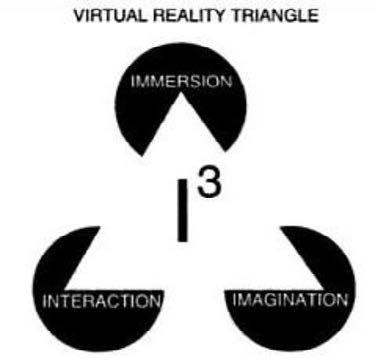
\includegraphics[width=0.30\textwidth]{3I}
    \caption{The 3I's of Virtual Reality - © 2003 by John Wiley \& Sons Inc. All rights
reserved}
    \label{fig:3I}
\end{wrapfigure}

1. \textbf{Immersion:} it is the virtual reality situation where the user feels personally inside the
scene and immerse inside the simulated virtual world.



2. \textbf{Interaction:} The interactive feedback between the user
and the virtual environment. Since it is a man-machine
interface, the system should promptly respond to the
user’s actions.


3. \textbf{Imagination:} The scene design and the construction of
the environment formulated with imagination for a
better user simulated experience.


  
  
  
The idea is to develop a new application to show Palestine with 360$^{\circ}$ videos, but it will include a part of one of the demolished villages before 1948. To rebuild one of those villages we need to know the structure of the village and how it looked like. The data about the structure of the village will be collected through personal stories, old pictures, British mandate aerial photos, and some maps made by a few people who lived in those villages. 
  
  
In the master project, a pre-study of the project will be conducted with Palestinians who live in the diaspora through interviews and workshops.  The Interview is a highly used method of collecting data in qualitative social research methods” \citep{Anyan2013}.  Kvale(1983)  described the purpose of as a method collection in social research as “... to gather descriptions of the life-world of the interviewee with respect to interpretation of the meaning of the described phenomena”  \citep{Kvale1983}. Semi-structured interviews will be used for collecting stories and exploring personal experiences about the Palestinians displacement and their relation with Palestine after living abroad. A questions guideline will be prepared for the interviews with  open-ended questions allowing a discussion with the interviewee rather than  formulated questions and answers.

After the interview some insights would be collected from the interviewee through a participatory design workshop. Participatory design (PD) is a set of theories, practices, and studies related to end-users as full participants in activities leading to software and hardware computer products and computer-based activities  \citep{Muller2003}. The field is extraordinarily diverse,  drawing on fields such as user-centered design, graphic design, software engineering, architecture, public policy, psychology, anthropology, sociology, labor studies, communication studies, and political science, and from localized experiences in diverse national and cultural contexts \citep{Gregory2003}.  Personal stories might give the ability for some refugees to draw the houses of their villages how they remember it. Applying a workshop for some of the Palestinian refugees to re-draw their houses would demonstrate a better image for the construction of the village, and that will give them the ability to tell us what they would like to see. houses, public places, walking paths between the houses, farms...etc. 
Information and communications technologies (ICT) artifacts should react to changing conditions of a social system \citep{Wulf2011}. Design case studies give us the ability to understand the relationship between social practice and the design of ICT artifacts that are built to support those practices, It is not so much about high tech, but about high-value \citep{Volker2013}. Design Case Studies ideally consist of three phases: (1) Analyze and particularly describe a social practice on a micro-level, as well describing the tools, media and their usage. (2) Describe the ICT artifacts from a product and from a process perspective, like the design concepts, and the applied design methods. (3) Document the introduction, appropriation and the potential re-design of the ICT artifact, documentation allows analyzing the trans-formative impact of certain functions and design options \citep{Volker2013}. Design case studies will allow us to check with the Palestinian refugees the tools or the practice that they do to see or to feel the connection with Palestine as a country and with their villages. After understanding their tools or practice, we can build a design depending on a specific design concept and methods. By letting them trying the prototype we will have general feedback about the interaction of the user with the App, and what would need to maintain and what kind of things needs to be re-designed. Design case studies will give us a general overview of the design concept and full fill us with the answers for the "how" and "why" about using the design methods.   
The Application will start by showing an overview of the whole map of historical Palestine. Points of interest will hover over the cities, the user will select a point of interest through the gaze feature. After selection, the map will be zoomed to the city location and will show more specified places within the city and the villages surrounding the city. The user will be transferred to a 360$^{\circ}$ video of the desired place, and inside the 360$^{\circ}$ video the user can commute inside the village for instance through the points of interest. sound of the surrounding environment will be added to the videos, as well as narrating the history and personal stories about the place. Within the demolished village, the user will have the ability to see how is the village look like now, and how it used to look like before 1948 by selecting an interactive button to travel in time. The user will have the ability to move back to the main map to choose to see different locations. All the methods that are used will help us to develop and collect the information and the data that is needed for the application and to be presented to the user.
\section{Related Work}
\section{Example projects}
\textbf{Auschwitz Virtual Tour}\footnote{Auschwitz VR Tour-\url{https://youtu.be/EOM_CxAKB_Y}}: The German broadcasting institution WDR made a 360o
documentary in Auschwitz concentration camp. Within the documentary, some Holocaust
survivors tell their stories. While listening to the stories and seeing the different locations in
the camp the user could feel the fear and horror that people suffered from. The video
immerses the user through the sound of the surrounding environment in the camp, you can
hear the wind and the sound gives a slight feeling of the cold weather over there. The
experience is immersive, but there is no interactivity with the user.


\textbf{Clouds over Sidra}\footnote{The Za’atari camp VR Tour-\url{https://youtu.be/mUosdCQsMkM}}: A 12 years old girls’ daily life story at the Za’atari refugee camp in Jordan
showed in virtual reality. The camp is a home for 80,000 Syrian refugees, half of them are
children(“Syrian Refugee Crisis – UN Virtual Reality,” 2015). The documentary was made by
the United Nation to raise awareness about the Syrian crisis. The video contained a number
of short videos from different parts of the camp, and it’s being synchronized while Sidra
narrates her story. It is more like watching a video with empathy than being immersed, but
the video presents the real life of the camp. Although the difference that while watching and
listening to the story, the user observes the people how they actually survive and live in the
camp. Therefore, the user does not have to imagine how is life over there.


\textbf{Carne y arena}\footnote{Carne y Arena Trailer-\url{https://youtu.be/zF-focK30WE}} : A highly professional
Virtual reality project that puts viewers
into the harsh life of an immigrant. The
user is placed among a group of
Mexican immigrants passing the
borders into the U.S. It was written and
directed by Alejandro G. Iñárritu. It Is a
full virtual reality experience; the user
needs to reserve an individual session
on the website. According to Pinotti (2017) you go in a dark room; your feet are on the sand (coarse grain, rough feeling) then, two assistants welcome you and provide you with the
necessary devices: an Oculus Rift headset, a backpack connected via cables to a powerful
computer and you are ready to be caught up in a nightmare \citep{Pinotti2017}. The project is
subtitled by ‘Virtually present, Physically invisible’. Pinotti (2017) defined, Virtually present:
“you are transported in the middle of the desert, among men, women, and children who try
their voyage of hope”. Physically invisible: “you are present, but nobody sees you and after a
while, you start to feel the need to be noticed and seek acknowledgment of social
recognition” \citep{Pinotti2017}. The project was developed with high technology, like 3D
modeling, visual effects, sound. The interaction of the user and the feeling of “being there”
by placing the user in a special environment, leads to a unique experience of immersion.


\chapter{Background}
\section{Virtual Reality}
Virtual reality is a technology which is often regarded as a natural extension to 3D computer graphics with advanced input and output devices \citep{Jayaram1997}. Ryan (2001) defined it as an “interactive, immersive experience generated by a computer” \citep{Ryan2001}. And according to G.C. Burdea and Coiffet (2017) “it is a generated computer graphics used to create a realistic-looking world that responds to the user’s input (gestures, verbal commands, etc.)” \citep{burdea2017virtual}. Virtual reality places the users inside the experience instead of viewing a screen in front of them, the users will be immersed inside a 3D world. As shown in Figure \ref{fig:3I} Three elements are needed to construct a virtual reality situation: immersion, interaction, and imagination. They are called the “3I’s” of virtual reality \citep{Hu2016}.


\begin{wrapfigure}{r}{0.30\textwidth} %this figure will be at the left
    \centering
    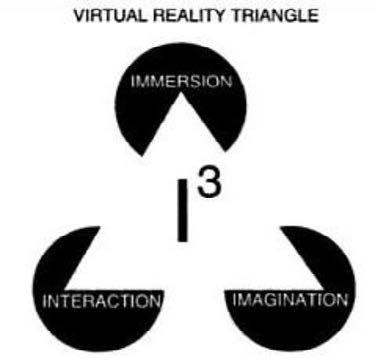
\includegraphics[width=0.30\textwidth]{3I}
    \caption{The 3I's of Virtual Reality - © 2003 by John Wiley \& Sons Inc. All rights
reserved}
    \label{fig:3I}
\end{wrapfigure}

1. \textbf{Immersion:} it is the virtual reality situation where the user feels personally inside the
scene and immerse inside the simulated virtual world.



2. \textbf{Interaction:} The interactive feedback between the user
and the virtual environment. Since it is a man-machine
interface, the system should promptly respond to the
user’s actions.


3. \textbf{Imagination:} The scene design and the construction of
the environment formulated with imagination for a
better user simulated experience.



\section{Political History}
Palestine, a country that is known by living in political conflict for decades.
The Zionist immigration to Palestine started in 1880's, with the ideology of rebuilding a national home for the Jewish people on their ancient land, the land of Israel, in Zionist parlance\citep{Morris2004}\citep{Pappe2006}.
Following the first Zionist Congress in Basel in 1897 at which the idea of
establishing a Jewish state in Palestine was first mooted, the rabbis of Vienna
dispatched two representatives to investigate the suitability of the country for
such an enterprise. The men reported the result of their explorations in this cable
to Vienna:




\centerline{\textit{\say{The bride is beautiful, but she is married to another man.}}}

This cable encapsulated the problem with which the Zionist movement had to grapple from the beginning: an Arab population already lived on the land on which the Jews had set their heart. The received view is that the Zionist movement, with the exception of a few marginal groups, tended to ignore the Arabs who lived in Palestine (Ghada Karmi)(Avi Shlaim).

\say{For many Zionists Palestine was not even an 
\say{occupied} land when they first arrived there in 1882, but rather an \say{empty} 
one, the native Palestinians who lived there were largely invisible to them or, 
if not, were part of nature's hardship and as such were to be conquered and 
removed. Nothing, neither rocks nor Palestinians, was to stand in the way of 
the national 'redemption' of the land the Zionist movement coveted} \citep{Pappe2006}.


Simultaneously, The Arab Revolution was forming during the last decades of the 19th century to gain 'Independence' from the Ottoman Empire. However, it became evident to some Palestinian leaders even before the First World War the potential for a future Jewish takeover of the country and the expulsion of the indigenous Palestinian people, it was recognized in the writings of the founding fathers of Zionism. Historical evidence shows that at some time between 1905 and 1910, 
several Palestinian leaders discussed Zionism as a political movement 
aiming to purchase land, assets and power in Palestine, although the 
destructive potential was not fully comprehended at that period. \citep{Pappe2006}.



 In 1917 and during The First World War the British government issued Balfour declaration that  announces the support to establish a \say{National home for the Jewish people in Palestine}. In the same year the Ottoman Empire was destroyed by the First World War and Britain conquered Palestine \citep{Morris2004}.  
 
 
 
 
 
 The British Mandatory over Palestine was approved in 1923 and Palestine was under the British mandate from 1923 to 1948. According to Sa’di \& Abu-Lughod
(2007) “on the last day of the mandate, the creation of the state of Israel was proclaimed,
and the 1948 Arab-Israeli war began” \citep{Sadi2007}. 

\begin{wrapfigure}{r}{0.20\textwidth} %this figure will be at the left
    \centering
    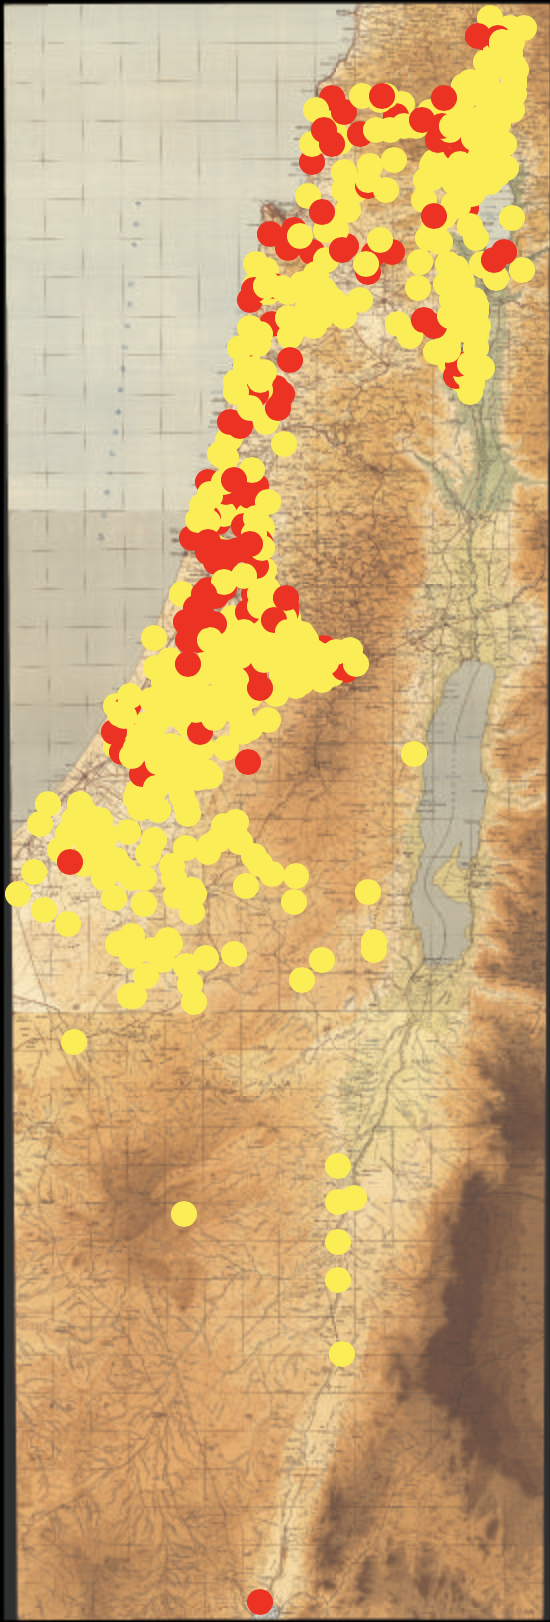
\includegraphics[width=0.20\textwidth]{d_villages}
    \caption{Demolished and depopulated villages - Palestine Open Maps, © 2018  Visualizing Palestine }
    \label{fig:map}
\end{wrapfigure}



The 1948 war that led to the creation of the State of Israel over Palestine also resulted in the devastation of the Palestinian society \citep{Sadi2007}. The day that Israel was created over Palestine, for Palestinians it was a catastrophe (“Nakba” in Arabic). At least 80\% of the Palestinians who lived in the major part of Palestine upon which Israel was established – more than 77\% of Palestine’s territory – became refugees. “The lives of the Palestinians at the individual,
community, and national level were dramatically and irreversibly changed” \citep{Sadi2007}.








The “Nakba” a massive number of Palestinians were deported outside of Palestine. “Of the
1,400,000 Palestinians in the country prior to the Nakba, just 150,000 individuals were listed
as being present during the first census carried out by the new Israeli state” \citep{Sanbar2007}.
According to Falah (1996) “Some of the Israeli military code names of their operations was
Matate (Broom), and Bi’ur Chametz (Passover Cleanup) – suggest that the war involved an
aspect of ethnic cleansing” \citep{Falah1996}\citep{Pappe2006}. The Israeli forces demolished and depopulated 531
Palestinian villages during the 1948 war, as shown in figure \ref{fig:map} the red dots represent the demolished villages, and the yellow dots represent the depopulated villages. According to the \acrshort{unrwa} in January 2015 registered
Palestinian refugees reached more than 5 million, divided between, The West Bank, Gaza
Strip, Syria, Lebanon, and Jordan \citep{DajaniDaoudi2011}. 

Since 1948 the Palestinian refugees are not allowed to return to Palestine, and not even for a visit. Due to the idea of the return of significant numbers of Palestinians to their villages and towns, or indeed to any part of Palestine, touches on deep-seated fears among Israelis regarding the legitimacy and permanence of the entire Zionist enterprise, as well as the Arab-Jewish demographic balance within Palestine \citep{Khalidi2016}. According to Pappé (2006), the Zionist organization and the Hebrew University mapped and made a detailed registry of all the Arab villages \citep{Pappe2006}.



The project of mapping the whole villages details turned out to be a "national Project" and it was called "The village files"\citep{Pappe2006}. In the late 1940's the "archive" was almost complete and the information became more explicitly military orientated \citep{Pappe2006}. In 2018 the Israeli national archive was published online, but after a time of research through the archive in English and in Hebrew, those maps and the detailed information about the villages were not openly published. according to Shezaf (2019), the Israeli defense minitsry secretive security department (Malmab) is responsible for concealing hundreds of documents as a part of a systematic effort to hide evidence of the Nakba.

%The website of the Israeli national archive, gave a form to fill explaining the reasons that the user needs to access such a data, without giving a clear answer if the user will get access to it. 
\section{Cultrual Identity}

\section{Al-Ghabisiyya Village}

Al-Ghabisiyya is located north east acre in distance of 11.5 km. The village stood on a rocky hill that jutted up from the plain of Acre. Judging from the many caves that were used as burial places, the area probably had been a large Canaanite town.
Al-Ghabisiyya was populated by 690 inhabitants, in 1931 it had 125 houses. The village was built in the late nineteenth century, it was inhabited by 150 residents back then\citep{Khalidi1992}.
\subsection{Al-Ghabisiyya before 1948}

 Al-Ghabisiyya was surrounded by a variety of trees like, olives, fig, and pomegranate. The village was near another two Villages Shaykh Dannun and Shaykh Dawud. Shaykh Dawud and Shaykh Dannun were overlapped at points, but Al Ghabisiyya was about 500m away from them. The entire population of these villages was Muslim. 

Al-Ghabisiyya had a school that was built by Ottomans in 1886. The village houses were built of reinforced concrete or, in some cases, stone held together with a mortar of mud or cement. The economy of the village was based on livestock raising and agriculture, grains and vegetables were the chief crops. the villagers also grow olives, which they processed on two animal-drawn presses, one in Al-Ghabissya and one in Shaykh Dawud.

In 1944/45 a total of 6633 dunums of the lands of the three villages was allocated to cereals, 1371 dunums were irrigated or used for orchards. In the same year 300 dunums in Al-Ghabisyya were devoted to olive trees\citep{Khalidi1992}.

\subsection{Occupation and Depopulation}

Al-Ghabisiyya fell at the end of operation Ben-Ami, the Haganah's invasion of the northwest corner of Palestine. The operation, which began 13-14 May 1948, was the last major Haganah offensive before the end of the British Mandate in Palestine. It was designed to capture all the coastal villages from Acre northwards to the Lebanese border\citep{Khalidi1992}.

In the words of Israeli historian Benny Morris, this was "in line with Plan D[alet]'s provision for securing blocks of Jewish settlement even outside the partition plan borders."\citep{Morris2004}

The Carmeli Brigade which carried out the operation, was given the order on 19 May 1948, "to attack in order to conquer, to kill among men, to destroy and burn villages of Al-Kabri, Umm al Faraj and Al-Nahr"\citep{Morris2004}. Al-Kabri was occupied the following night, on 20-21 May, as part of the second stage of operation Ben-Ami. Along with a series of villages in western Galilee, north of Acre, Al-Nahr was captured 20-21 May 1948, during this second phase of the opertation. Units of the Carmeli Brigade attacked Al-Ghabisiyya it was the last village taken on 20-21 May 1948. Al-Ghabisiyya surrendered formally and that some of its population were expelled sometime during the following days or weeks\citep{Morris2004}.

The attack was waged from two directions, the north and southeast. The occupying forces captured a house in the southernmost corner of the village and proceeded to shell the village from the house, killing and injuring many of the villagers while they were fleeing. Others had been evacuated earlier, due to the fall of Acre. The village militia decided to not confront the Zionist forces because they were too few (around twenty) and very poorly armed. Most of those who were driven out remained in other villages in Galilee until the whole region fell at the end of October 1948, after that they were displaced to Lebanon\citep{Khalidi1992}.

Some inhabitants remained in Al-Ghabisiyya until Febrauary 1949. During that month, there was a second explsionm this time by the Military Government, on grounds of "security and order". it is not clear where they expelled villagers were taken\citep{Morris2004}.

After Al-Ghabisiyya and its two neighboring villages of Shaykh Dannun and Shaykh Dawud were evacuated, the Israeli government permitted some of the inhabitants of the latter two villages to return to their homes. Those who had not sought refuge in Lebanon came back and were joined by a few families from Al-Ghabisiyya, Al-Nahr, Al-Tall, Umm Al-Faraj, 'Amqa, and Kuwaykat. The two small villages of Shaykh Dannun and Shaykh Dawud were merged to form a joint village called Shaykh Dannun, in 1973 it had a population of about 1000. The Village of Al-Ghabisiyya was not repopulated \citep{Khalidi1992}.  

\subsection{The Village Today}

The only landmark that remains is the mosque, a doomed, stone structure, with arched doors and windows and decorative arches in the interior. It is deserted, the cement plaster on the doom is peeling off, and wild shrubs cover the rest of the roof. The debris of houses, terraces, and the village cemetery can be seen among a thick forest of cypress trees that was planted on the village site and part of the land. Cactuses also grow on the site. The settlement of Netiv ha-Shayyara that was established by Iraqi Jewish immigrants in 1950, uses the adjacent non-forested land for agriculture.    

\section{The YALLAH! Hackathon}

\acrshort{yallah!} Is a student’s exchange research program between the University of Siegen in
Germany and Birzeit University in Palestine funded by the DAAD. The program was
constructed for a collaboration between students to create social innovation projects.
In \acrshort{yallah!} 2018 there were three different projects Mobile Makerspace, VR Experience and
\acrshort{yallah!} Computer Club. The \acrshort{yallah!} program is divided into three phases: The preparation
phase (boot camp), a research phase in Germany, and an implementation phase in Palestine.
The \acrshort{yallah!} Hackathon preparation phase
The participants of \acrshort{yallah!} learned about some research methods and how to apply them in
the projects through a boot camp week. During the boot camp, the teams took their first
steps in the projects by planning the research track, setting a research question, and building
a strategy to achieve their goals.
The Palestinian and the German students attended the boot camp separately, therefore the
boot camp took a place once in Germany and another time in Palestine. The purpose of the
boot camp was to introduce and train the participants on the research methods (such as how
to make interviews, how to take field notes, and how to observe while working in the field).
The students split up into 3 groups each group studied one method through literature and
then presented it to the other participants. By the end of the presentation, the students
discussed the method together and practiced it inside the group. The boot camp was very
good practice for the methods and emphasized the research skills of the participants. At the
boot camp in Germany, the Virtual reality project students made their first test in filming with
a 360o camera, they used the Samsung Gear 360 camera to record part of the boot camp
sessions in a purpose to use it later in the project as a testing video. Due to the average video
quality of the Samsung Gear 360 camera, the VR students added a task to their list that is to
find a 360o camera with better quality. The students also discussed the interesting spots in
Palestine related to the historical and religious places mentioned in biblical stories.
The \acrshort{yallah!} Hackathon research phase
The Palestinian students visited Germany for the research phase. The Palestinian and the
German exchange students met in Siegen, Germany for the first time. The students gathered
on the first day and had an introduction from the supervisors about the whole \acrshort{yallah!}
program in general and the research phase in Germany. After the introduction on the first
day, the teams of each project gathered and discussed their plans for the research and the
implementation phases. The VR team members discussed the kind of methods to be used in
the research, the team decided on Interviews and Thinking Aloud as methods for collecting
data from random people and from Palestinians who live in Germany. Therefore, there were
multiple tasks needed to be done by the team to start working with those methods. The VR
team split the tasks among the members: creating the interview questions guideline,
documentation, building a prototype, and logistics, for instance, to create a contact list of
interesting people to contact and have an interview with them.
After one month after the end of the research phase, the VR team had their second gathering
in Palestine to start the implementation phase. The implementation phase contained a lot of
filming in different places in Palestine. Depending on the research results and the discussion
with the team members, they created an organized plan for visiting different places in
Palestine and capturing the area using the camera. The plan included the main cities of
Palestine, famous touristic sightseeing locations and religious places since people showed
high interest to see those spots. Therefore, the team recorded in Jerusalem, Jaffa, Haifa, Akka
(Acre), Ramallah, Nablus, Jericho, Hebron, and Bethlehem.
\subsection{VR Application development}
\chapter{Methodology}
In this section, I outline the methodological approach and the steps that I took to form and adjust the concept of the design. Frameworks like Design Case Studies and Action Research were leading the project to a journey of collecting results, planning, acting and reflecting on the project. Ethnographic Research methods like interviews and field notes enhanced the documentation process and quick feedback. 

\section{Design Case Studies}

Design Case Studies is a research framework that is divided into three phases Pre-study, Design and Appropriation \citep{Wulf2011}. These phases allow the researcher to understand the relationship between social practices and the space of designing IT artifacts to support these practices \citep{Volker2013}. The Pre-study phase is a context study for understanding social practices, and participatory ethnographic studies where the researcher requires close collaboration with practitioners \citep{Rohde2017GroundedPerspective, Wulf2011}. I conducted interviews with Palestinian refugees/immigrants in Germany, meanwhile, I did a literature review, and I researched for the existing applications or platforms that are related to Virtual reality in Palestine, also I studied the results of the research that was conducted during \acrfull{yallah!} hackathon. The Design phase focuses on the design concept of the artifact and how its influenced by the changes in social practices or how the design can enhance existing practices. Therefore, ethnographic analyses are required to determine the potential for a suitable new artifact \citep{Rohde2017GroundedPerspective, Wulf2011}.
\begin{figure}[ht]
    \centering
    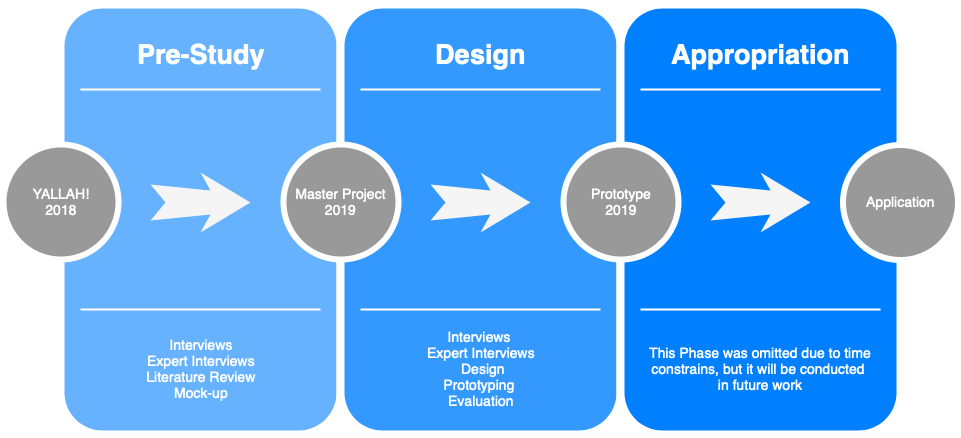
\includegraphics[width=0.90\textwidth]{images/DCS_Diagram.png}
    \caption{Design Case studies Timeline}
    \label{fig:dcs}
\end{figure}


In the Design phase I analyzed the data that I collected in the Pre-study. I designed a prototype and conducted expert interviews for obtaining feedback. Then I tested it with users and received an evaluation from them. The Appropriation phase is to analyze the impact of ICT artifact on the transformation towards social practices\citep{Wulf2011}. The researcher will be able to observe the effect of the design on the practice through a certain amount of time. I omitted the Appropriation phase due to time constraints but it will be conducted in further future work with the application.   


\section{Action Research}

Kurt Lewin sometimes called \say{The father of action research}\footnote{The real father of action research is Jacob L. Moreno (1892-1974) who developed the idea in Germany in the 1920s.} described action research in terms of a cycle of steps of planning a change \citep{KemmisSdanMcTaggart1988}.
Action research is a framework that enables the researcher to investigate and evaluate his work \citep{Khanna2007AllResearch}. Also, it is specifically cooperative, interdisciplinary, and interactive. Action research primary focuses on iterative action on the research implementation process for ICT artifacts or any other process, the significant measures are the research results and the viability of the artifact. A spiral cycle that contains planning, acting, observing and reflection, it enables the researcher to take action and observe the results and then to reflect and take action again and so on \citep{Hayes2011TheInteraction}. 
\begin{figure}[ht]
    \centering
    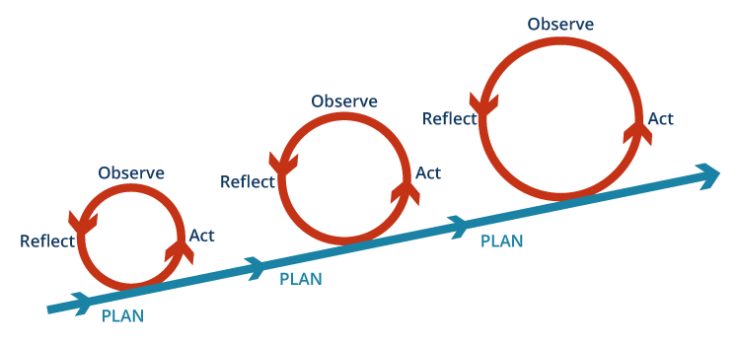
\includegraphics[width=0.90\textwidth]{images/par.png}
    \caption{Action Research steps - © wiobyrne.com  }
    \label{fig:par}
\end{figure}

This \say{spiral of action research} is now familiar to many people. Action research is hardly as smooth as implies this sequence of self-contained loops of planning acting observing and reflecting. The stages intersect, and in the light of learning from experience, initial plans easily become redundant. The process is likely to be faster, more transparent and more adaptive \citep{KemmisSdanMcTaggart1988}. I made several enhancements on the application through the pre-study phase e.g. \acrfull{ui} it had significant enhancements after I observed the actions and reflected on them, and that implies the whole application as well.     


\section{Qualitative Ethnographic Research Methods}

In the following section, I will define some Ethnographic methods that I conducted through the research. I will also present how I used those methods to gather qualitative data from the field and the user. I conducted several interviews with multidisciplinary people in Germany and Palestine, followed by expert interviews to get a wider view of Virtual Reality from experts. I also took some notes during my trip to Palestine and I will explain it as a method and in the next sections.        

\subsection{Interviews}

“The Interview is a highly used method of collecting data in qualitative social research methods” \citep{Anyan2013}. \cite{Kvale1983} described the purpose of the interview as a method of data collection in social research as “...to gather descriptions of the life-world of the interviewee with respect to interpretation of the meaning of the described phenomena” \cite[p.174]{Kvale1983}. Interviews can provide perspectives and useful data from participants. An important source of insights is by having a conversation with the right participants and interact with them. 
Three types of interviews are unstructured interviews, semi-structured and fully structured interviews \citep{Lazar2017ResearchInteraction}. Unstructured interviews are more like a free-form conversation, without any planned questions or guidelines. A semi-structured interview is using established questions that were planned out, but the interviewer can ask additional follow-up questions as the interviewer see it appropriate and not only commit to the questions guideline. This loose structure and the open-ended interview are benefits for collecting additional insights in the interview \citep{Pannafino2017UXMethods}. A fully structured interview is a more quantitative research method where the interviewer follows the flow of the structured questions in the guideline to obtain data about a specific objective usually employed in survey research. Therefore, direct conversations with participants can provide qualitative data that a survey can miss \citep{Lazar2017ResearchInteraction}. \say{If you don't listen to your users, you might miss some of the most important feedback that you can get} \cite [p.187]{Lazar2017ResearchInteraction}. Although the surveys can validate the findings of the interviews within a large population of \citep{Pannafino2017UXMethods}. During the interview, the interviewer needs to listen carefully and take notes while deciding which comments to pursue. It is better to also record the interview with the participant's consent, therefore, the interviewer can refer back to the interview later and use it to analyze the data. Analysis of raw-notes and recorder interviews is a challenge because of deciding which is good data and which is bad, then the interviewer will generate a key of findings depending on the theme or pattern that he followed \citep{Lazar2017ResearchInteraction, Pannafino2017UXMethods}.
I conducted twelve semi-structured and open-ended interviews with multi-disciplinary people in Germany and Palestine, six of the interviews were with privileged second and third Palestinian refugee/immigrant generations living in Germany, two interviews with refugees from Al-Ghabisiyya village and another two interviews with Palestinian refugees in the Westbank. One interview with a high school student from Ramallah, and another interview with a senior man from Jerusalem. Nine of those interviews were recorded and the participants signed a declaration of consent, the rest of the interviews were not recorded due to some technical difficulties but I took notes during all the interviews. Then I transcript all the interviews and analyzed all the data and got major insights that were clear and came from all the participants.           

\subsection{Expert Interview}
The expert interview was designed to explore expert knowledge, it is a qualitative research method. Only the researcher decides whom to conduct an interview with as an expert. Expert Interviews according to \cite{Christmann2016}  “in scientific research an individual is addressed as an expert because the researcher assumes – for whatever reason – that she or he has knowledge, which she or he may not necessarily possess alone, but which is not accessible to anybody in the field of action understudy” \cite[p.18]{Christmann2016}. Although, Experts knowledge must be unique and not accessible by everyone, otherwise it wouldn't be considered as expertise. \say{An expert is someone who is responsible in some way or another for the development, implementation or monitoring of a problem or who has privileged access to information about people or decision processes} \cite[p.221]{Christmann2016}. Conducting the expert interview in purpose to explore a certain phase in a project would be concentrated and efficient for gathering data in a short time. As well it will be easier and faster to obtain good results from the expert interviews. I conducted two informal interviews with experts, hence it was more like an intellectual conversation and I gained data and experience from those interviews, the first interview was with a Virtual Reality expert, and the second one was with an expert in the Palestinian villages and stories about the Palestinian Nakba \say{Catastrophe}. None of these interviews were recorded, but notes were taken by paper and pen. 

\subsection{Field Notes}

Field notes are a necessary part of the ethnographic research. Researchers take notes during observations and conversations in the field, they are defined as a shorthand reconstruction of events. Researchers and ethnographers decide about what they want to write about while they are in the field \citep{Wolfinger2002OnExpectancies}. Those decisions that are taken by researchers and ethnographers are usually unarticulated and invisible to the reader. The field notes would construct the field trip with brief narratives from the moment that the researcher enters the field to the moment he leaves while the field site is not confined in a particular location. The researcher must take notes about every single detail not only through the interview but about the artifacts, the landscape the surrounding circumstances also events on the ground. Not all the data should be always formally documented, researchers and ethnographers should also pay attention to the unrecorded or not captured moments during the fieldwork \citep{Boulus-rdje2018StuckSite}. I took notes while I was conducting interviews, I was writing notes from the participants but I also was writing their reactions, if they were getting excited or emotional. During the field trip, I tried to take as many notes as possible, but I always wrote all the notes by the end of the day when I arrive home.   

\section{Prototyping}

A prototype is an initial representation of a design that is made in a purpose of testing before producing the final artifact \citep{Buchenau2000ExperiencePrototyping}. Prototyping is the core factor for exploring and testing the designs for interactive systems. Prototypes will evaluate the new design and examine it, as well as present the problems in the design \citep{Buchenau2000ExperiencePrototyping, Houde1997WhatPrototype}. Despite which medium the designer is using, a prototype can always represent the design idea. Three dimensions are important for any interactive design: role, look and feel, and implementation. The role is asking about how the artifact is useful for the user's life. Look and feel, questions the experience of the user and what the user sees and feels or hears from the artifact. Implementation refers to the functionality of the artifact and how does it work. The prototype might present design options from one or two or three dimensions of the model \citep{Houde1997WhatPrototype, Buchenau2000ExperiencePrototyping}. I built a prototype that contained a 360$^{\circ}$ video from Damascus gate in Jerusalem. The prototype was a mobile application that I implemented on my smartphone and I used Google daydream \acrshort{vr} glasses to let the users try it. later on, I enhanced the prototype with a better interface. The interface helped the users to see different locations of the city. The prototype gave me good insights from the users and gave the users a better idea about the application.

\section{Thinking Aloud}

Thinking aloud is commonly used in digital platforms for usability testing \citep{VanWaes2000}. The thinking-aloud approach consists of making a user interact with a computer system (prototype, paper mock-up or documentation),  automatically users start expressing thoughts, data, intentions, opinions, hopes, fears, anxieties, etc.  Thinking aloud is a process that provides participants with a model in a situation and is often tested by participants reflecting on how they use the prototype. Each verbalization is transcribed and then analyzed in a formal analysis process. In the context of the informal guidelines, observers are asked to take note of what the participants say and do without attempting to interpret their actions and words, particularly where they encounter difficulties \citep{Jrgensen1990}. There are two kinds of thinking aloud techniques, retrospective think-aloud, and concurrent think aloud. Retrospective think-aloud is a specific situation is recorded or verbalized after the experience. Concurrent think-aloud it is handled while the users are experimenting with a specific task, like solving a problem, surfing the web or navigating a \acrshort{vr} environment \citep{Friedman2004NavigatingSteps}. According to \cite{Marsh1999EvaluationUsability} the main difference between a two-dimensional digital interface and \acrfull{vr} system, that the evaluation happens from inside the \acrshort{vr} environment. Thinking aloud in \acrshort{vr} applications measure the user performance on two levels, the user performance with the \acrshort{vr} application, and the behavior of the user inside the \acrshort{vr} application \citep{Marsh1999EvaluationUsability}. I conducted thinking aloud sessions after each interview with the participants, I
took notes while I was observing the users behavior in the \acrshort{vr} application. By following
a concurrent think-aloud type, users were asking me questions and sometimes I asked
them to do some specific tasks. After the participants finish exploring the application, I asked them for their feedback and to evaluate it.  






\chapter{Application Development}


\section{Virtual reality components}



A \acrshort{vr} system is made up of two major subsystems, the hardware and software. The hardware can be further divided into \acrshort{vr} engine and I/O devices, while the software can be divided into application software and database as illustrated in Figure \ref{fig:sys}.
The classical five components of a \acrshort{vr} system are, Software and Database, \acrshort{vr} Engine, I/O Devices, User and Task \citep{burdea2017virtual,Bamodu2013VirtualComponents}.

\begin{figure}[ht]
    \centering
    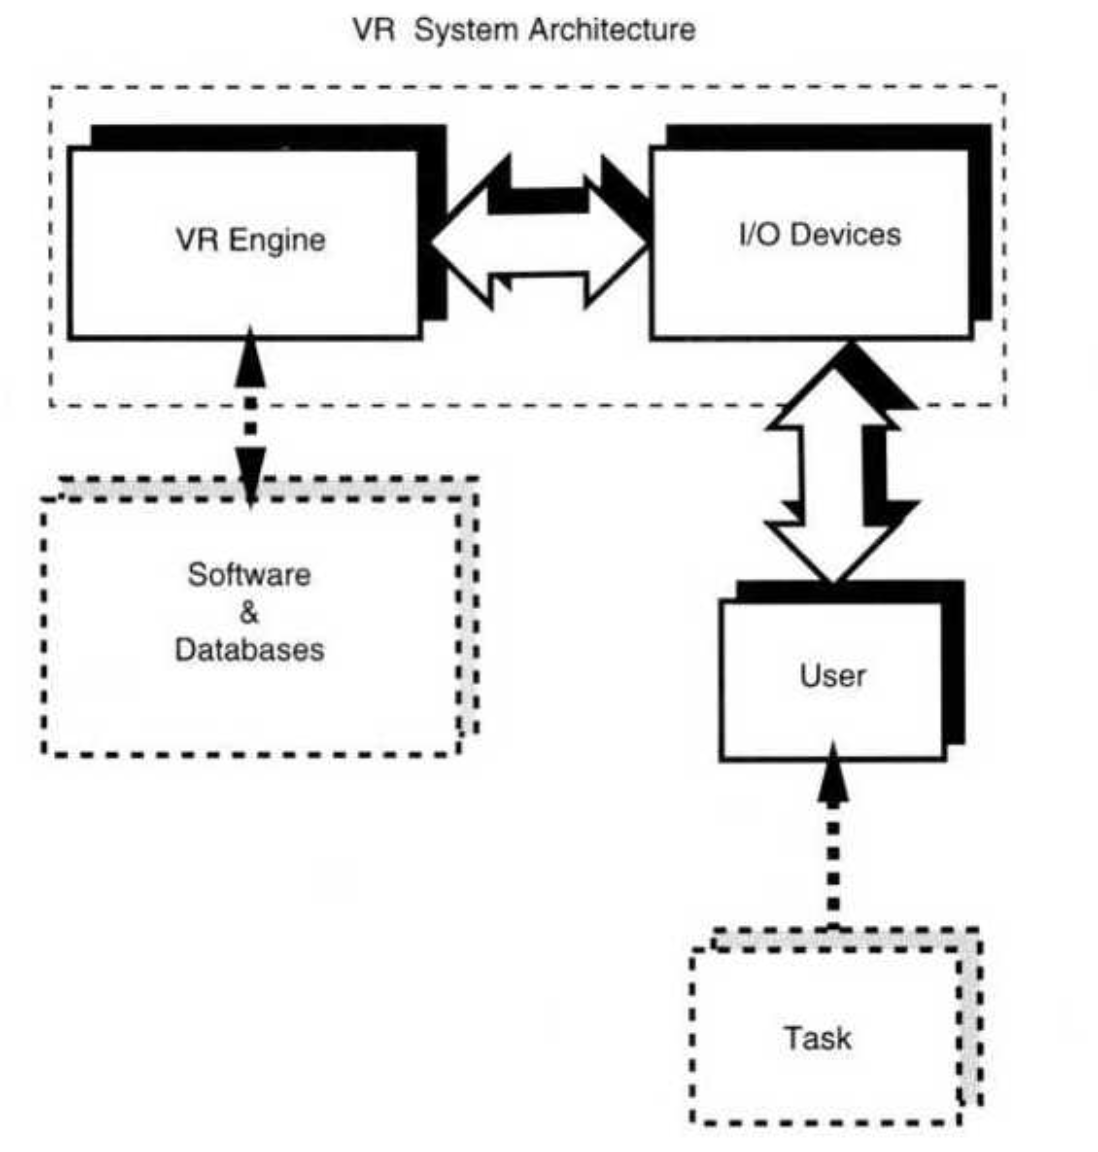
\includegraphics[width=0.50\textwidth]{images/VR.png}
    \caption{VR System Architecture - \citep{burdea2017virtual}}
    \label{fig:sys}
\end{figure}


\subsection{Software and Database}
Virtual reality system software is a colletion of tools and software for designing, developing and
maintaining virtual environments and the database where the information is stored. The tools can be classified into modeling tools and development tools.

VR Modeling Tools. There are many modeling tools available for VR designing, the most
common ones are , 3ds Max, Maya and Creator. Engineering specific applications might use software like CATIA, Pro/E, Solidworks, UG, etc. VR Development Tools. VR is a complex and integrative technology that borrows from many other technologies, such as real time 3D computer graphics, tracking technology, sound processing, and haptic technology, among others, therefore software development flexibility and real time interaction is needed.


\subsection{VR Engine}
VR Engine. In VR systems, the VR engine or computer system has to be selected according to the
requirement of the application. Graphic display and image generation are some of the most important factors and time consuming task in a VR system. The choice of the VE engine depends on the application field, user, I/O devices, level of immersion and the graphic output required, since it is responsible for calculating and generating graphical models, object rendering, lighting, mapping, texturing, simulation and display in real-time. The computer also handles the interaction with users and serves as an interface with the I/O devices. A major factor to consider when selecting the VR engine is the processing power of the computer, and the computer processing power is the amount of senses (graphical, sound, haptic, etc) that can be rendered in a particular time frame as pointed. The VR engine is required to recalculate the virtual environment approximately every 33ms and produce real time simulation of more than 24fps [4], furthermore, the associated graphic engine should be capable of producing stereoscopic vision. The VR engine could be a standard PC with more processing power and a powerful graphics accelerator or distributed computer systems interconnected through high speed communication network.


\subsection{I/O Devices}
Input Devices. The input devices are the means by which the user interacts with the virtual world. They send signals to the system about the action of the user, so as to provide appropriate reactions back to the user through the output devices in real time. They can be classified into tracking device, point input device, bio-controllers and voice device. Tracking devices sometimes referred to as position sensors, are used in tracking the position of the user [1], and they include, electromagnetic, ultrasonic, optical, mechanical and gyroscopic sensors, data gloves, neural and bio or muscular controllers [2]. Examples of point-input devices include 6 DOF mouse and force or space ball. Their technology is an adaptation of the normal mouse with extended functions and capability for 3D. Voice communication is a common way of interaction among humans. So it feels natural to incorporate it into a VR system. Voice recognition or processing software can be used in accomplishing this.

Output Devices. The output devices get feedback from the VR engine and pass it on to the users through the corresponding output devices to stimulate the senses. The possible classifications of output devices based on the senses are: graphics (visual), audio (aural), haptic (contact or force), smell and taste. Of these, the first 3 are frequently used in VR systems, while smell and taste are still uncommon.
Two possible common options for the graphics are the stereo display monitor, and the HMD which provides a higher level of immersion. In the HMD, the two independent views produced are interpreted by the brain to provide a 3D view of the virtual world. Audio or sound is an important channel in VR; its importance is only surpassed by that of visual. 3D sound can be used in producing different sounds from different location to make the VR application more realistic.
Haptic is used to allow the user feel virtual objects. This can be achieved through electronic signals or mechanical devices.



\subsection{User}



\subsection{Task}



\section{Hardware and Development Environments}

In this section, I will mention and define the equipment and tools that I used to develop the application. Also, I will present how I did manage to re-build part of the Al-Ghabisiyya village. These tools helped me in modeling the terrain of the geographical area as well as re-building some of the houses around the mosque of Al-Ghabisiyya. Placing the village on the right location of the map was tricky and challenging therefore, I will explain it in detail. 
\subsection{Headsets}

\textbf{Google Cardboard}: The virtual reality platform was released in
2014 by Google. The platform is intended as a low-cost system to
encourage interest and development in VR applications. It was
named for its fold-out cardboard viewer. The Google Cardboard
headsets are built out of simple, low-cost components -
cardboard. Google open-sourced the schematics and the
assembly instructions freely on their site, allowing people to
assemble Cardboard themselves from readily available parts (“Google Cardboard,” 2014). The
cardboards were the best option to be used for the project due to the easy mobility and the
low price. It is easier to travel with it through airports or checkpoints since it’s cardboard.
\subsection{Cameras}
\textbf{GoPro Fusion}: the footage quality can reach up to 5.2K spherical video
resolution. The GoPro fusion can be controlled via a mobile
application through Bluetooth or Wi-Fi. The two lenses on the two
sides are not symmetrically aligned, they are off-axis. That helps to
process the images or the footage taken from the two lenses to not
have visible stitching or overlapping in the final image. That is a
common problem in most of the VR cameras to have a big overlapping on the final image. The
data is saved on two microSD cards one for each lens, the files need to be combined to have
a final 360o video \citep{Easton2018}. The camera was used in most of the project filming material,
it has the best footage quality and a perfect stabilization in the videos.


\textbf{Samsung Gear 360}: The small and rounded shape of the camera is ideal for
handheld shooting, although it has a socket also for a tripod. A small LCD
screen helps in navigating through the camera modes. The video resolution is
4K, while the still images are somewhat soft. The smartphone app is easy to
use and clear for the user also it offers a good range of viewing options. In
general is it a small and simple camera to use (Digital Camera, 2018). The
camera used as a backup camera during the project. The quality is acceptable
for a small and very light camera.

\subsection{Development Environments}

The VR technology is moving forward and there is an increasing number of tools and platforms
available for developers (“11 Tools for VR Developers,” 2017). VR technology has found its
way into different environments like computers, smartphone, and web. This section will
mention the two tools that were used by the VR team developers to build a mobile VR
application and a VR experience over the web. Nevertheless, most browsers are still struggling
with the headset device support. Most phones can be detected with the WebVR-polyfill and
if turned sideways, it will switch the dual display mode automatically that you can use Google
Cardboard or other headsets built for smartphones (“11 Tools for VR Developers,” 2017).


\textbf{Unity 3D}: Unity is one of the most famous game engines, it has a direct VR mode to preview
the work on any Head mounted display, which can be easier and faster for designers to boost
their productivity. Most of the Head mounted displays are supported in Unity. Unity works
with C\# and JavaScript; it is easy to learn due to the huge online community. Unity can export
the work to almost any platform even WebGL (“11 Tools for VR Developers,” 2017). Unity was
the best and most powerful tool to be used during the project to develop the VR experience.
Due to the easy implementation of the VR Environment in Unity, also the variety of platforms
that it allows the developer to distribute the software on it. In addition, there is a huge
community for Unity developers on the internet, where everyone can share knowledge and
expertise.

\section{Development \& Implementation}



\subsection{Glimpses from Palestine Application}





\subsection{User Interface}

“ In order to allow human-computer interaction it is necessary to use special interfaces designed to input a user's commands into the computer and to provide feedback from the simulation to the user” \citep{burdea2017virtual}.
\chapter{Results}

\section{Preliminary Empirical Research Findings}
\section{On The Ground Research Findings}
\section{Reflection on UX Design}
\section{Evaluation of Glimpses from Palestine Application}
\chapter{Discussion}
I will discuss the results and the challenges of the research in this chapter. The results have been collected during interviews in the pre-study phase in Germany and the Design phase in Palestine. Those results came along together after designing the application. Nevertheless, there were challenges during the research phases, I will mention them in detail in the second section of this chapter. 

\section{Discussion Results}
In this research, I wanted to check if Virtual Reality can let people overcome borders. During the pre-study, the results showed the need of the users and the connection that they have for the country.  Also, during \acrshort{yallah!}, the results were showing that people thought about Palestine that its only a war zone. The Palestinians in the diaspora also showed a lot of interest to know and see their country. They are highly connected to the country, but they also do not know how it looks like. The participants showed that they got their identity and their connection to Palestine only through their grandparent's and parent's stories. But also they got connected through the struggle cause of the Palestinians, and the unfairness that they face daily. Multiple links connect the people with the country. The grandparents who were deported out of Palestine, they have like a romantic relationship with Palestine. In the way that they described the country for their kids and grandchildren. It is described as heaven but the children would have different imaginations. That's the effect of why one of the participants told me that he didn't want to see the house that it belongs to his grandparents in the village because maybe it doesn't look like the image that he has for it in his head. Glimpses from Palestine give the ability for the user to experience the real-life in Palestine, from the struggle to the normal life in different places. I need to let people see what the real-life in Palestine, instead of being scared to go to Palestine and be exposed to danger. Glimpses from Palestine would be a safe platform to experience life safely. Also, it has the feature of time traveling for getting more historical facts and stories about how Palestine looked like before 1948. Al-Ghabisiyya is one of 536 villages, and in every village, there is a different story.  



\section{Challenges}

As with every project, during development, there are several obstacles. I faced challenges during the development of the application and during my fieldwork. During the development process, I confronted difficulties in programming due to some functionalities like opening and closing panels for the user. I didn't have any prior knowledge about how to build and open a new interface for the user within VR. I developed the Application on Unity on the 2018 version, but that version was not compatible with the Plug-in that is responsible for building the terrain. To create the Al-Ghabisiyya terrain, I had to download Unity 2019 update. At the end of creating the final results, I combined the two projects in one file. That created a series of errors, and I needed to fix them. They were fixed and I installed the first copy of the application on my smartphone. Thus, I was able to do the usability test with it. 
Collecting the data about the villages, in general, it was a challenge. There wasn't a lot of sources about the details of each town. Maps were almost impossible to reach, even the Ariel photos that were taken by the British Mandate.  The map that I received had no orientation or scaling key. Therefore, collecting the data and the maps to implement them and rebuild a village or a town it was very challenging. However, my connections from the field made it easier for me. I believe it would be even more difficult for someone who wasn't raised in Palestine or at least not from the same culture. I am Palestinian and I speak the language, and I found that challenging. To be able to collect data and insights the interviewee needs to trust the interviewer. Nevertheless, people in Palestine are not easy to trust anybody, especially when the conversation is about politics. Multiple people refused to be interviewed after I introduced them to the topic. They are from the West Bank refugee camps. There is no easy way to build trust with the refugees, they need to know you personally. Fortunately, I knew and interviewed refugees from the camps. I needed to interview also Palestinian refugees in the diaspora camps. The majority of Al-Ghabisiyya inhabitants were deported to Lebanon. I have no access to be in Lebanon physically, due to law restrictions on the Lebanese borders toward Palestinians. I have a contact in Lebanon, and in the refugee camps, she knew some people. She made contact with a man who once lived in Al-Ghabisiyya. That was another challenge, I was worried about the trust factor, but apparently, the man was happy about the interview and by talking to me while I am in Palestine. It was another behavior that could be influenced by the country's love and passion.  When I went to Al-Ghabisiyya It was a long trip therefore, my time there was limited. While I was there I had to conduct interviews and film the location in 360$^{\circ}$ degrees videos, before the time of the last train goes back to Jerusalem. One of the lenses in the camera did not function. I had to disassemble it and fix it while being there. Fortunately, it worked and I filmed the whole area successfully. 
\chapter{Limitation}
This chapter will address the limitations that I encountered during my research. There were technological constraints during the development of the application. And there were also restrictions on the ground, by collecting data and documentation. In the first section, I will talk about the technological boundaries and in the second section, I will display the restriction on the maps in Palestine. 
 

\section{Technology}

Developing the application with the large capacity of videos showed the limitations of my computer. The videos were rendered and prepared every night, but the consequences were to fill the hard drive with data. However, I saved all the videos on external hard drives and I made a daily backup for my laptop data.  At some point, my laptop stopped working, it didn't restart and not even load a safe mode. I tried all the possibilities but nothing worked. I started to restore the data from the backup drive. After retrieving all the data back, and replace the lost data. Unfortunately, the Android \acrfull{sdk} in Unity didn't function anymore. Therefore I couldn't install the new copy of the application on my smartphone. The copy would include Al-Ghabisiyya in \acrshort{vr} after building it, also a lot of other scenes from the country. Technology here limited me and time constraints as well because it was the last week for me in the field and I needed to let users test the Application. Luckily I had the previous copy of the application on my smartphone, and I showed the users the village on the laptop how did it look like. 
   

\section{Access to Maps}

The maps in Palestine are very unique, even with the new technologies that we have. Google maps, for instance, have a lack of information about the Palestinian areas at the West-bank. That also implies to those demolished villages there is no information related to them. The maps or even pictures for these villages are very complicated and very rare to find. As I mentioned in the Background chapter, the Israeli government blocked all this data from being published. This limited me to obtain more information and maps to reconstruct the other villages. The map of Al-Ghabissiya was taken by the British mandate from an ariel photo. If I had access to ariel photos or maps I would have constructed more villages in Virtual Reality. 
\chapter{Conclusion and Future Work}
\input{chapters/Conclusion.tex}


\bibliographystyle{apalike}
\bibliography{references}
\appendix
\chapter{Declaration of Consent}



\textbf{Project: Glimpses of Palestine}


Declaration of consent for sound, image and video recordings



I,-------------------------------------- , have been informed orally by Samer Shawar that sound, image and video recordings of me will be made as part of the above project.

The recordings serve exclusively to view and analyze the evaluation again. They are recorded with a recording device and then potentially written down by the staff of the research project.

There is a chance I am recognizable in the footage. For this reason, all persons involve in the evaluation are subject to absolute confidentiality. The recordings will not be passed on to third parties.

I am aware that my statements in scientific papers are quoted in excerpts, and I was assured that they will be treated anonymously. Image extracts, on which I am shown, are anonymized before a possible publication. All information that could lead to the identification of my person will changed or removed from the text.

Since I can potentially be recognized in the recordings, I have the right to have these recordings deleted at any time without any disadvantages. To get recordings of me deleted, I contact the researcher.

The declaration of consent for sound, image and video recordings is voluntary. I can revoke this declaration of consent at any time. In the event of rejection or withdrawal, I will not incur no costs or other disadvantages. However, participation in the study will then not be possible.

Personal contact data are stored separately from interview data and are inaccessible to third parties. After completion of the research project, I have been assured that my contact data will be automatically deleted, unless I expressly agree to further storage for the contact option for topic-related research projects. I can object to longer storage at any time.

Participation in the research in voluntary. I may at any time cancel an interview, refuse further participation and withdraw my consent to a recording and transcript without any disadvantage to me.

\vspace{5mm}
I agree to take part in an interview/several interviews, workshops, and focus groups as part of the research project mentioned above.


 $\Box$ Yes \hspace{15mm}
 $\Box$ No

\vspace{10mm}
I agree to be contacted for future related research projects. For this my contact details about the end of the research project remain stored.


 $\Box$ Yes \hspace{15mm}
 $\Box$ No


\vspace{10mm}
I have received a copy of this declaration of consent.


 $\Box$ Yes \hspace{15mm}
 $\Box$ No



\vspace{5mm}
For question or other concerns, I can contact the following: 


Samer Shawar


Kohlbettstrasse 15


D-570072 Siegen


samer.shawar@student.uni-siegen.de

\vspace{15mm}

--------------------------------------------------  \hspace{20mm}            ---------------------------------------------


Place, Date and Signature of Participant	\hspace{15mm}         	Name of Participant in Block letters
\vspace{10mm}

--------------------------------------------------  \hspace{20mm}            ---------------------------------------------


Place, Date and Signature of Researcher	\hspace{15mm}         	Name of Researcher in Block letters


\end{document}

